\section{Design Exploration} 
\label{sec:design_exploration}

In this section, we study the variability in IPSs that can violate a predefined fixed threshold. 
We then investigate how existing approaches fail or become inefficient under this variability, and explore the potential of an adaptive thresholding scheme. 

\subsection{Variability in Intermittent Systems} 
\label{subsec:dynamic_energy_consumption}
 
Design-time profiling of workloads' energy consumption in the prior work can be potentially violated by the variability of IPSs.
To study and demonstrate the variability, we chose the built-in AES accelerator on the TI MSP430FR5994 microcontroller unit (MCU) as an example peripheral workload.  
The example AES function encrypts data in the cypher block chain mode, and can process up to 4KB data with a 128-, 192-, or 256-bit key length. 
In the following experiments, we measured $\Delta \symb{V}{task}$, \textit{the drop of supply voltage caused by an operation without any incoming energy meanwhile}, which directly determines the minimum voltage threshold that safely guarantees the completion of an atomic operation. 
We used Device 1 in Table~\ref{tab:device}, which has \SI{11.5}{\micro\farad} energy buffering capacitance, for the tests for variable data sizes and peripheral configurations, whereas in the device variability test we tested 3 devices.
We explored four factors that can possibly change $\Delta \symb{V}{task}$, which are variable data amounts, variable peripheral configurations, devices variability, and capacitor degradation and tolerance. 
Besides the above four, energy consumption can also change with other factors, such as temperature, clock frequency, and silicon ageing, but we have found them either insignificant or hard to validate on our experimental platform. 


% 22 uF extra capacitance, or 33 uF extra capacitance
% the MCU board has a 10 + 1.5 uF capacitance


\subsubsection{Variable Data Sizes}

A peripheral function can accept a runtime variable amount of data, such as a variable data size to encrypt or different lengths of packets for a radio to transmit. 
An example of this is plotted in Figure~\ref{fig:variable_datasize}, where the size of the square dots represent a \SI{5}{\milli\volt} precision error of the scope and the lines represent linear regression. 
We observed that $\Delta \symb{V}{task}$ has a linear relationship with the data size, with an offset energy consumption that accounts for the initialisation. 
%The dynamic range of $\Delta \symb{V}{task}$ is \SIrange{17}{194}{\milli\volt}.
In this case, the linearly scaled $\Delta \symb{V}{task}$ comes from linearly scaled run time. 

\begin{figure}[!t]
    \centering
    \begin{tikzpicture}
    \pgfplotsset{set layers}
    \begin{axis}[
        scale only axis,
        width=0.7\columnwidth,
        height=4cm,
        ymin=0,ymax=200,
        xmin=0,xmax=4,
        axis y line*=left,
        y axis line style={Set1-A},
        xlabel=Data Size to Encrypt (KiB),
        ylabel=$\Delta V_{\text{task}}$ (mV),
        legend style={at={(0.05,0.95)},
        anchor=north west,legend columns=1},
        ]
        \addplot
            plot [Set1-A,only marks,mark=square]
            table [x=data_size, y=voltage_drop,col sep=comma] {ch5_optic/figures/variable_data/variable_data.csv};
            \label{delta_V_task}
        \addplot
            plot [Set1-A]
            {44.31027668 * x + 16.926383399209485};
        % \legend{$\Delta V_{\text{task}}$}
    \end{axis}
    \begin{axis}[
        scale only axis,
        width=0.7\columnwidth,
        height=4cm,
        ymin=0,ymax=7,
        xmin=0,xmax=4,
        axis y line*=right,
        y axis line style={Set1-B},
        axis x line=none,
        ylabel=Run Time (ms),
        legend style={at={(0.95,0.05)},
        anchor=south east,legend columns=1},
        ]
        \addlegendimage{/pgfplots/refstyle=delta_V_task}\addlegendentry{$\Delta V_{\text{task}}$}
        \addplot
            plot [Set1-B,only marks,mark=o] 
            table [x=data_size, y=time,col sep=comma] {ch5_optic/figures/variable_data/variable_data.csv};
            \addlegendentry{Run Time}
        \addplot
            plot [Set1-B]
            {1.60436561 * x + 0.07670306324110676};
        % \legend{Run Time}
    \end{axis}
    \end{tikzpicture}
    \caption{$\Delta V_{\text{task}}$ varying linearly with the data size in AES 128-bit encryption.}
    \label{fig:variable_datasize}
\end{figure}


\subsubsection{Variability in Peripheral Configurations}

A peripheral can run with variable configurations at runtime, and demonstrate variable performance and energy consumption. 
For example, as shown in Table~\ref{tab:configurations}, an AES accelerator can encrypt data with 128-, 192-, or 256-bit keys. 
A longer key provides higher security, but also takes more time and energy to complete.
The dynamic range of configuration variability in this case can be a 26\% increase in $\Delta \symb{V}{task}$ and a 33\% increase in run time.
% Can refer to "A control flow" for the need of runtime configurations

\begin{table}
    \renewcommand{\arraystretch}{1.2}
    \centering
    \caption{$\Delta \symb{V}{task}$ Varying with Configurations in AES 4KB Encryption}
    \label{tab:configurations}
    \begin{tabular}{|c|c|c|}
    \hline
    \textbf{Configuration} & \textbf{$\Delta \symb{V}{task}$} & \textbf{Run Time} \\
    \hline
    128-bit key & \SI{583}{\milli\volt} & \SI{6.479}{\milli\second} \\
    192-bit key & \SI{690}{\milli\volt} & \SI{7.638}{\milli\second} \\
    256-bit key & \SI{736}{\milli\volt} & \SI{8.606}{\milli\second} \\
    \hline
    \end{tabular}
\end{table}

\subsubsection{Device Variability}

Devices have their variation in power consumption, even with the same part number. 
A threshold profiled on one device can be inadequate on another. 
We did a test on three developments boards of the same MCU, where it runs 128-bit AES encryption on 4KB data. 
As listed in Table~\ref{tab:device}, the effect of device variability on $\Delta \symb{V}{task}$ is up to 9\% among the three devices, though with almost the same run time (0.5\% variation). 
% This has been moderated by the larger on-board capacitance on Device 1 -- the actual charge consumption is supposed to be 31\% larger than Device 3.
It should be noticed that device variability can also present across platforms that can run the same or similar code. 

\begin{table}
    \renewcommand{\arraystretch}{1.2}
    \centering
    \caption{$\Delta \symb{V}{task}$ Varying among Devices in AES 128-bit 4KB Encryption}
    \label{tab:device}
    \begin{tabular}{|c|c|c|}
    \hline
    \textbf{Device No.} & \textbf{$\Delta \symb{V}{task}$} & \textbf{Run Time} \\
    \hline
    % 1 & \SI{764}{\micro\ampere}\\
    % 2 & \SI{773}{\micro\ampere}\\
    % 3 & \SI{756}{\micro\ampere}\\
    1 & \SI{583}{\milli\volt} & \SI{6.479}{\milli\second} \\
    2 & \SI{555}{\milli\volt} & \SI{6.444}{\milli\second} \\
    3 & \SI{535}{\milli\volt} & \SI{6.462}{\milli\second} \\
    \hline
    \end{tabular}
\end{table}

\subsubsection{Capacitor Ageing and Tolerance}
\label{subsubsec:capacitance_variability}

As the component for buffering energy in IPSs, capacitors typically present a $\pm$10-20\% tolerance on rated capacitance as reported in many commercial capacitors. 
Capacitors also age over time. 
It is shown that capacitance can decrease by 7.2\% in 3000 hours (125 days) under a \SI{25}{\celsius} ambient temperature in experiments~\cite{kulkarni2010experimental}, and by 50\% within 10 years under \SI{40}{\celsius} as manufacturers stated~\cite{vishaycapacitor}.
A degraded capacitor does not change the load consumption, but can increase $\Delta \symb{V}{task}$, and hence makes the pre-defined voltage threshold unsafe or inefficient. 


The above four examples present that the variability in IPSs can potentially make a predefined $\Delta \symb{V}{task}$ insufficient. 
It is unrealistic to profile the $\Delta \symb{V}{task}$ in each scenario at design time in practice considering the complexity of the variations, and still cannot encompass unexpected situations, necessitating a runtime energy profiling approach. 


% Simulation
\subsection{Performance Improvement with Adaptive Thresholds}

Having presented the variability in IPSs, we explore in modelling and simulation the potential of adaptive thresholds on coping with such variability, as opposed to existing fixed-threshold approaches, which may fail or run inefficiently under such variability.

% i.e. the system always set the lowest possible threshold for the next operation.

\subsubsection{Power Analysis}

As suggested in prior work, operating at a lower voltage can improve system energy efficiency due to a higher charging efficiency and a lower power consumption.

To validate this, we analysed the charging characteristic of a glass-type amorphous PV panel in an white LED lighting environment. 
We used the PV panel to charge a \SI{103}{\micro\farad} capacitor from \SI{0}{\volt} to \SI{3.05}{\volt} where the capacitor cannot be charged up anymore. 
The voltage-time charging trace is then differentiated to gain an I-V curve that represents the PV panel (\fref{fig:pv_iv}). 
% The scattered dots do not line up in a smooth curve thanks to the precision error of the scope. 
To model this curve, we did a linear regression for the data in \SIrange{0}{2.3}{\volt}, and adapted a published PV panel model~\cite{en9050326} to represent the curve in \SIrange{2.3}{3.05}{\volt}.
The model function of this I-V curve is then expressed as:
\begin{equation}
    \nmm{I}{in} = \left\{
    \begin{aligned}
        & -16.25 \nmm{V}{in} + 276.10 & , & \quad \SI{0}{\volt} < \nmm{V}{in} <= \SI{2.3}{\volt} \\
        & \nmm{I}{sc} (1 - e ^ {ln(1 - \frac{\nmm{I}{mpp}}{\nmm{I}{sc}}) \frac{\nmm{V}{in} - \nmm{V}{oc}}{\nmm{V}{mpp} - \nmm{V}{oc}}}) & , & \quad \SI{2.3}{\volt} < \nmm{V}{in} <= \SI{3.05}{\volt}
%         I_sc * (1 - math.exp(math.log(1 - I_mpp / I_sc) * (v - V_oc) / (V_mpp - V_oc)))
    \end{aligned}
    \right. 
    \quad (\SI{}{\micro\ampere})
    \label{eq:pv_iv}
\end{equation}
where we set \nm{I}{sc} = \SI{276}{\micro\ampere}, \nm{V}{oc} = \SI{3.05}{\volt}, \nm{I}{mpp} = \SI{237}{\micro\ampere}, and \nm{V}{mpp} = \SI{2.3}{\volt}.

\begin{figure}
    \centering
    \begin{tikzpicture}
    \begin{axis}[
            width=0.9\columnwidth,
            height=7cm,
            ymin=0,
            ymax=300,
            xmin=0,
            xmax=3.1,
            xlabel=Voltage (V),
            ylabel=Current (\SI{}{\micro\ampere}),
            legend style={at={(0.05,0.05)},
            anchor=south west,legend columns=1},
        ]
        \addplot
            plot [black,only marks]
            table [x=v, y=i,col sep=comma] {ch5_optic/figures/pv_curve/pv_curve.csv};
        \addplot
            plot [gray,ultra thick,domain=0:2.3,on layer=foreground]
            {-16.25 * x + 276.10};
        \addplot
            plot [gray,ultra thick,domain=2.3:3.05,on layer=foreground]
            {276 * (1 - e ^ (ln(1 - 237 / 276) * (x - 3.05) / (2.3 - 3.05)))};
        \legend{Measurements, Model Fitting}
    \end{axis}
    \end{tikzpicture}
    \caption{An I-V curve of a glass-type amorphous PV panel (Sanyo AM-1417CA, \SI{35}{\milli\meter}$\times$\SI{13.9}{\milli\meter}) under a white LED lighting condition.}
    \label{fig:pv_iv}
\end{figure}

In the MSP430FR5994 platform, we did not observe a significant change in current consumption with supply voltage (up to 2\%). 
This is majorly due to an on-chip LDO that droops down the external supply voltage to a constant internal supply voltage, and hence maintaining a relatively stable current draw as the external supply voltage changes. 
Hence, we omitted the voltage effect on current consumption in this simulation. 

We used the energy and time overheads of AES encryption presented in \sref{subsec:dynamic_energy_consumption} to simulate the workload characteristics. 
In simulation, the current draw remains constant during one operation, but changes with dynamic data sizes and configurations due to the variable charge consumption and run time.

\subsubsection{Runtime Control Models}

We modelled an ideal adaptive threshold scheme against two SoA fixed-threshold schemes.
We focussed on modelling the control logic and threshold settings, and omitted the state management overhead as it can be dependent on the actual implementation. 

In the ideal adaptive scheme, the system knows exactly how much energy is needed for the next operation and sets the lowest threshold that suffices the energy budget. 

\debs{} sets a minimum threshold for a fixed operation. 
We explored two cases of \debs{}, labelled as \debs{} Low and \debs{} High.
We firstly modelled \debs{} Low, which does not foresee any possible changes in data sizes and configurations. 
\debs{} Low's threshold was profiled with 1KB data and a 128-bit key length without considering any variability. 
We then modelled \debs{} High in a case where it foresees the possible dynamic increase in workload consumption due to variable data sizes and configurations and sets its threshold based on the most energy-hungry setup, while it does not consider further capacitor ageing.
% Unfortunately, \debs{} Low fails to achieve any progress except for few operations at the beginning of the simulation given origin capacitance.
% Thus, we use \debs{} High to represent \debs{} in the following results.

Samoyed differs from \debs{} and the adaptive scheme in its control, where, when completing an operation, it keeps executing until it dies rather than sleeps and waits for the next threshold.
Samoyed suggests allocating an abundant energy budget, so its threshold is also set to the highest possible operating voltage.

% DEBS High is probably not the most efficient DEBS. 
% An efficient DEBS can have multiple, but a limited number of, thresholds. 
% This is a bit unfair.

\subsubsection{Simulation Setup}

In simulation, the system has \SI{10}{\micro\farad} system capacitance without charge at the start. 
The shutdown threshold is \SI{1.8}{\volt}, against which \debs{} and the adaptive scheme set their threshold, with a \SI{10}{\milli\volt} small margin. 
The system consumes \SI{10}{\micro\ampere} when it is inactive.
To evaluate the performance of the three schemes, we conducted two tests that simulate a variable workload and capacitance reduction respectively.  
The variable workload test runs a random data amount from 16B to 4080B (1 to 255 blocks of data, 16B per block), and also a random 128-, 192-, or 256-bit key length, both uniformly distributed. 
The energy harvesting characteristics presented in \fref{fig:pv_iv} is used as the supply for this test. 
All the schemes take the same random series of data sizes and configurations.
The capacitance reduction test runs with 0-60\% reduced capacitance, in line with the maximum possible reduction shown in \sref{subsubsec:capacitance_variability}.
The system in this test is supplied with a \SI{50}{\micro\ampere} constant current and runs only the most energy-hungry operation, in order to examine whether the system can avoid non-termination even under the worst case.  
We ran 10 rounds of simulations for each setup, and each round simulates for \SI{10}{\second}. 

\subsubsection{Results}

% Separate figures
% \input{figures/exploration_results/failures.tex}
% \input{figures/exploration_results/completions.tex}
% Figure~\ref{fig:failure}
% Figure~\ref{fig:completion}

% Grouped figure
%\begin{figure}[t]
    \centering
    \begin{tikzpicture}
    \begin{groupplot}[
        group style={group size=1 by 2,vertical sep=10pt,x descriptions at=edge bottom},
        width=1.0\columnwidth, height=4.5cm,
        ybar,
        ymin=0,
        enlarge x limits=0.3,
        legend style={at={(1,1.07)},
            anchor=south east,legend columns=-1,
            /tikz/every even column/.append style={column sep=0.2cm}},
        legend image code/.code={
            \draw [#1] (0cm,-0.1cm) rectangle (0.2cm,0.25cm);},
        xlabel={Reduction of Capacitance},
        symbolic x coords={0\%,30\%,60\%},
        xtick=data,
        tick align=inside,
        ]
        \nextgroupplot[ymax=60,ylabel={No. Completions},]
        % DEBS low
        \addplot
            plot [black,fill=Set1-A,postaction={pattern=dots},error bars/.cd,y dir=both,y explicit]
            table [x=cap_reduct,y=debs_l_perf,y error plus=debs_l_perf+, y error minus=debs_l_perf-, col sep=comma] {ch5_optic/figures/exploration_results/results.csv};
        % Samoyed
        \addplot
            plot [black,fill=Set1-B,postaction={pattern=north east lines},error bars/.cd,y dir=both,y explicit]
            table [x=cap_reduct,y=samoyed_perf,y error plus=samoyed_perf+, y error minus=samoyed_perf-, col sep=comma] {ch5_optic/figures/exploration_results/results.csv};
        % DEBS high
        \addplot
            plot [black,fill=Set1-C,postaction={pattern=north west lines},error bars/.cd,y dir=both,y explicit]
            table [x=cap_reduct,y=debs_h_perf,y error plus=debs_h_perf+, y error minus=debs_h_perf-, col sep=comma] {ch5_optic/figures/exploration_results/results.csv};
        % REPA
        \addplot
            plot [black,fill=Set1-D,postaction={pattern=grid},error bars/.cd,y dir=both,y explicit]
            table [x=cap_reduct,y=repa_perf,y error plus=repa_perf+, y error minus=repa_perf-, col sep=comma] {ch5_optic/figures/exploration_results/results.csv};
        \legend{\debs{} Low, Samoyed , \debs{} High , Adaptive}

        \nextgroupplot[ymax=30,ylabel={No. Failures},]
            % DEBS low
        \addplot
            plot [black,fill=Set1-A,postaction={pattern=dots},error bars/.cd,y dir=both,y explicit]
            table [x=cap_reduct,y=debs_l_fail,y error plus=debs_l_fail+, y error minus=debs_l_fail-, col sep=comma] {ch5_optic/figures/exploration_results/results.csv};
        % Samoyed
        \addplot
            plot [black,fill=Set1-B,postaction={pattern=north east lines},error bars/.cd,y dir=both,y explicit]
            table [x=cap_reduct,y=samoyed_fail,y error plus=samoyed_fail+, y error minus=samoyed_fail-, col sep=comma] {ch5_optic/figures/exploration_results/results.csv};
        % DEBS high
        \addplot
            plot [black,fill=Set1-C,postaction={pattern=north west lines},error bars/.cd,y dir=both,y explicit]
            table [x=cap_reduct,y=debs_h_fail,y error plus=debs_h_fail+, y error minus=debs_h_fail-, col sep=comma] {ch5_optic/figures/exploration_results/results.csv};
        % REPA
        \addplot
            plot [black,fill=Set1-D,postaction={pattern=grid},error bars/.cd,y dir=both,y explicit]
            table [x=cap_reduct,y=repa_fail,y error plus=repa_fail+, y error minus=repa_fail-, col sep=comma] {ch5_optic/figures/exploration_results/results.csv};
    \end{groupplot}
    \end{tikzpicture}
    \caption{Numbers of completed and failed operations among four control schemes given random data sizes and configurations under three capacitance conditions. }
    \label{fig:simulation}
\end{figure} 


\fref{fig:simulation_perf} shows the mean, maximum, and minimum numbers of completed and failed operations in the variable workload test. 
\debs{} Low cannot terminate once it encounters an operation that consumes more than what it is profiled for and the supply is too weak to provide the energy gap. 
\debs{} Low can only occasionally get progress on lightweight operations before non-termination. 
Samoyed also suffers performance loss from waiting for a high energy threshold (\SI{2.9}{\volt} in this case), and failing an operation at the end of an active cycle. 
\debs{} High is relatively efficient because it does not usually fail due to a suffcient energy budget and a sleep-after-completion control. 
The adaptive scheme runs the most efficiently among these four.
It runs at reduced operating voltage that improves system energy efficiency, and also guarantees the completion of every task by setting a minimised but safe threshold.
As an example voltage trace shown in \fref{fig:simulation_voltage}, the adaptive scheme runs with \SI{2.11}{\volt} mean voltage, while the ones for Samoyed and \debs{} High are \SI{2.36}{\volt} and \SI{2.40}{\volt} respectively. 
Due to the above reasons, the adaptive scheme completes more operations over Samoyed by 50\% and \debs{} High by 15\% on average.

\begin{figure}
    \centering
    \begin{tikzpicture}
    \begin{groupplot}[
        group style={group size=1 by 2,vertical sep=40pt},
        width=0.9\columnwidth,height=5cm,
        xbar,
        symbolic y coords={debsl,samoyed,debs,adaptive},
        xmin=0,
        enlarge y limits=0.2,
        tick align=inside,
        ytick style={draw=none},
        yticklabels={,\debs{} Low,Samoyed, \debs{} High, \nn{} Oracle},
        ]
        \nextgroupplot[xmax=600,xlabel={No. of Completions}]
        \addplot
            plot [black,fill=Set1-B,error bars/.cd,x dir=both,x explicit]
            table [y=method,x=perf,x error plus=perf+,x error minus=perf-,col sep=comma] {ch5_optic/figures/exploration_results/perf.csv};

        \nextgroupplot[xmax=60,xlabel={No. of Failures}]
        \addplot
            plot [black,fill=Set1-A]
            table [y=method,x=fail,col sep=comma] {ch5_optic/figures/exploration_results/perf.csv};
        \node [anchor=west, font=\footnotesize, Set1-A] at (axis cs:0,adaptive) {0};
        \node [anchor=west, font=\footnotesize, Set1-A] at (axis cs:0,debs) {0};
        \node [anchor=west, font=\footnotesize, black] at (axis cs:0,debsl) {Non-Termination};

    \end{groupplot}
    \end{tikzpicture}
    \caption{Numbers of completed and failed operations of \debs{} Low, Samoyed, \debs{} High, and \nn{} Oracle given random data sizes and configurations and a PV supply in a \SI{10}{\second} simulation. }
    \label{fig:simulation_perf}
\end{figure} 

\begin{figure}
    \centering
    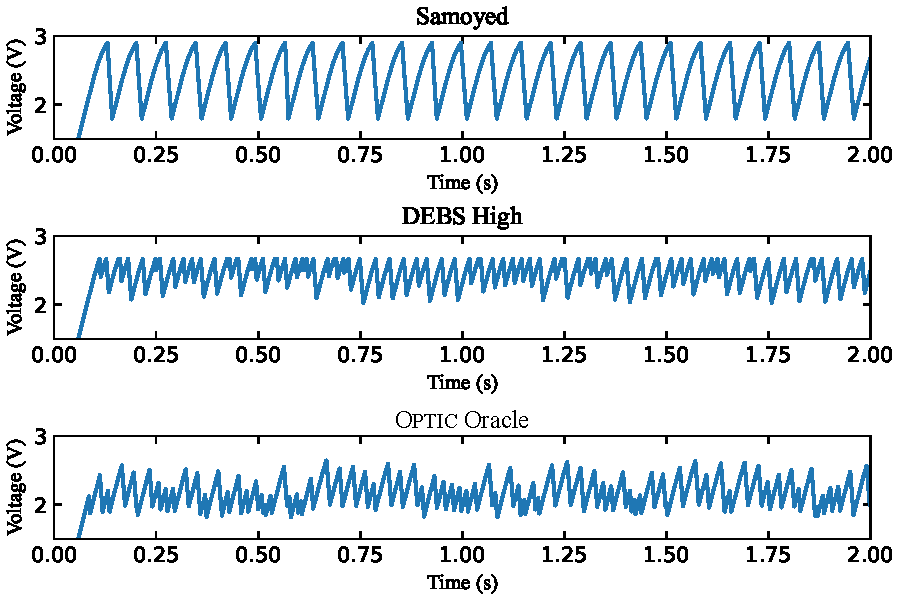
\includegraphics[width=\columnwidth]{ch5_optic/figures/voltage_traces.pdf}
    \caption{An instance of supply voltage traces in simulation. }
    \label{fig:simulation_voltage}
\end{figure}

\begin{figure}
    \centering
    \begin{tikzpicture}
    \begin{axis}[
        width=0.8\columnwidth,height=5cm,
        ymin=0,ymax=50,
        xmin=0,xmax=60,
        xlabel={Capacitance Reduction},
        ylabel={No. of Completions},
        xticklabel={\pgfmathprintnumber\tick\%},
        xticklabel shift={3pt},
        legend style={
            anchor=south,
            at={(0.5,0.1)},
            legend columns=3,
        },
        ]
        \pgfplotstableread[col sep=comma]{ch5_optic/figures/exploration_results/cap.csv}{\mytable};
        \addplot 
            plot [Set1-A,mark=triangle*,dashed]
            table [x=cap_reduction,y=samoyed_perf] {\mytable};
        \addplot 
            plot [Set1-B,mark=square*,dashed]
            table [x=cap_reduction,y=debs_perf] {\mytable};
        \addplot 
            plot [Set1-C,mark=*,dashed]
            table [x=cap_reduction,y=repa_perf] {\mytable};
        \legend{Samoyed,\debs{} High,Adaptive}
    \end{axis}
    \end{tikzpicture}
    \caption{Number of completed operations of Samoyed,\debs{} High, and the Adaptive scheme with capacitance reduction. }
    \label{fig:simulation_cap}
\end{figure}

\fref{fig:simulation_cap} shows the results of the capacitance reduction test, where we have omitted \debs{} Low as it has already failed in non-termination with origin capacitance (so will still fail with reduced capacitance). 
With the capacitance decreased, \debs{} High also falls into non-termination like \debs{} Low. 
Samoyed, where its threshold is set to \SI{3.6}{\volt} in this case, can still progress until a 60\% reduction of capacitance because its abundant energy budget can support at least one or a few operations in one active cycle.
The adaptive scheme still maintains the highest forward progress among these control scheme. 


The above exploration presents that using a fixed low threshold can leave the system in non-termination (e.g. \debs{} Low and \debs{} High) but allocating an abundant energy budget compromises system efficiency (\debs{} High and Samoyed). 
An adaptive threshold can potentially overcome both problems.

Motivated by the previous examples of variable energy consumption and the benefit of an adaptive threshold, we propose \nn{}, a new methodology for profiling energy consumption of tasks at runtime and adapting energy budgets to the variable energy consumption of tasks. 
